% !TEX TS-program = xelatex
% !TEX encoding = UTF-8 Unicode
% !Mode:: "TeX:UTF-8"

\documentclass{resume}
\usepackage{zh_CN-Adobefonts_external} % Simplified Chinese Support using external fonts (./fonts/zh_CN-Adobe/)
%\usepackage{zh_CN-Adobefonts_internal} % Simplified Chinese Support using system fonts
\usepackage{linespacing_fix} % disable extra space before next section
\usepackage{cite}
\usepackage[hidelinks]{hyperref}
\usepackage{fontawesome5} % 加载图标包
\usepackage{enumitem} % 确保已加载enumitem宏包
\usepackage{fontspec}
\usepackage{graphicx}
\usepackage[absolute,overlay]{textpos}
\setmainfont{Times New Roman}
\setmainfont[
  Path = fonts/Main/ ,
  Extension = .otf ,
  UprightFont = *-regular ,
  BoldFont = *-bold ,
  ItalicFont = *-italic ,
  BoldItalicFont = *-bolditalic ,
  SmallCapsFont = Fontin-SmallCaps
]{texgyretermes}


\begin{document}
\pagenumbering{gobble} % suppress displaying page number
% 右上角的图片
\begin{textblock*}{0mm}(\paperwidth-38mm,0mm) % 调整 textblock 的大小和位置
    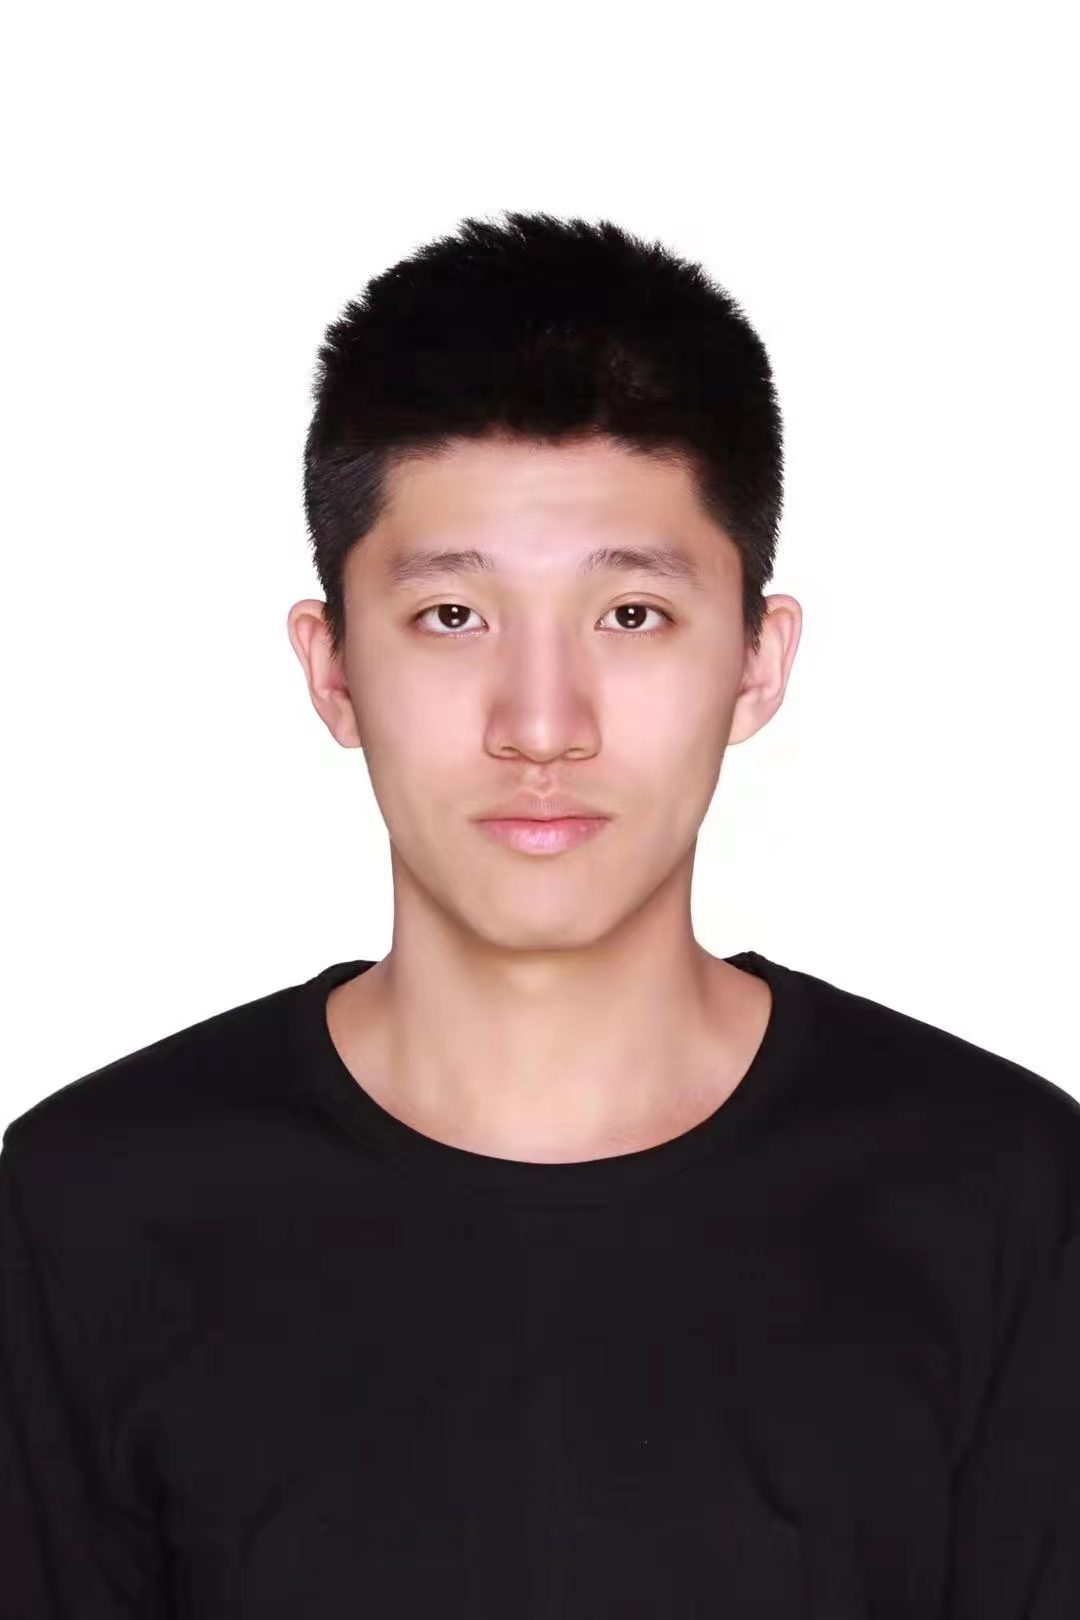
\includegraphics[width=25mm,height=25mm]{CHN/resume-master/生活照.jpg}
\end{textblock*}


\name{王雷}


 
% {E-mail}{mobilephone}{homepage}
% be careful of _ in emaill address

\begin{center}
    \faPhone \ \small  \underline{+86-15004513389} \quad % 使用 fontawesome5 的图标
    \href{mailto:lwang925@uwo.ca}{\faEnvelope \ \underline{lwang925@uwo.ca}} \quad % 邮箱超链接
    \href{https://www.linkedin.com/in/lei-wang-uwo/}{\faLinkedin \ \underline{www.linkedin.com/in/lei-wang-uwo/}} \quad % LinkedIn 超链接
    \href{https://github.com/LeiWangUog/}{\faGithub \ \underline{https://github.com/LeiWangUog}} % GitHub 超链接
    \end{center}
% {E-mail}{mobilephone}
% keep the last empty braces!
%\contactInfo{xxx@yuanbin.me}{(+86) 131-221-87xxx}{}
 

\vspace{-7pt}
% \section{\faGraduationCap\ 教育背景}
\section{教育背景}
\datedsubsection{\textbf{英国格拉斯哥大学},\textbf{金融学},\textbf{理学硕士}}{2023.9 - 2024.6}
\begin{itemize}[itemsep=0.2ex, parsep=0ex]
\item\ \textbf{绩点:GPA 3.5} 
\item\ \textbf{主修课程:Matlab 金融工程, Python机器学习,实证资产定价,金融衍生品定价}

 \end{itemize}
 \vspace{-5pt}
\datedsubsection{\textbf{加拿大西安大略大学},\textbf{金融管理},\textbf{管理学学士}}{2018.9 - 2022.6}
\begin{itemize}[itemsep=0.2ex, parsep=0ex]
\item\ \textbf{绩点:GPA 3.8},
\item\ \textbf{校内奖项:2018-2021三个年度校内奖学金,2020校内学术成绩优秀奖,三次Dean's Honor List(前10\%)}
\item\ \textbf{主修课程:会计学,金融学 ,宏微观经济学,资产定价,管理学,经济计量,统计学,精算学}
 \end{itemize}
 \vspace{-7pt}
% \section{\faCogs\ IT 技能}
\section{技术能力}
% increase linespacing [parsep=0.2ex]
\begin{itemize}[parsep=0.2ex]
  \item \textbf{编程语言}: MATLAB, Python (熟练), Stata, SQL
  \item \textbf{技术}: Scikit-Learn, PyTorch, TensorFlow, Pandas, NumPy, Matplotlib
  \item \textbf{机器学习算法}: CNN,RNN,GAN,MLP,决策树,随机森林,XGBoost
  \item \textbf{工具}{: \LaTeX{}, VS Code, Anaconda, MySQL, Microsoft Excel VBA, Bloomberg, WRDS, Capital IQ.} 
  \item\textbf{语言}{: 英语 (熟练), GRE 310, IELTS 6.0}
  \item\textbf{证书}{: 证券从业资格证,基金从业资格证,BMC彭博数据终端} \\
\end{itemize}

\vspace{-18pt}
\begin{1.5}
\section{工作经历}
\datedsubsection{\textbf{立达信物联科技股份有限公司 | \textit{Leedarson}},\textit{总裁办,证券事务专员}}{2023.2-2023.9}
\begin{itemize}[itemsep=0.5ex, parsep=0.3ex]
  \item \textbf{负责投资者关系等相关工作内容};具体为接待保荐人日常审查,投资机构分析师以及上市公司协会等调研,负责公司展厅及产品讲解,上交所业绩说明会,互动易平台回复、IR邮箱查询回复、官网IR页面搭建和更新。
  \item \textbf{负责公司对外信息披露};具体为完成公司2022年年度报告、中期报告、季度报告及企业社会责任报告(CSR)和起草并记录三会材料。独立完成公司年报中股权结构;股东信息;限售和非限售股;募集资金使用情况;资产减值等财务内容,并及时向上交所披露。
\end{itemize}

\datedsubsection{\textbf{北京利安达会计师事务所 | \textit{Reanda}},\textit{管理咨询部,审计员}}{2022.6-2023.2}
\begin{itemize}[itemsep=0.5ex, parsep=0.3ex]
  \item \textbf{独立负责2022年中国中冶集团武汉三家子公司的内控与风险管理监督评价工作。}具体职责包括:负责对中国一冶、中冶南方以及武汉勘察设计院的采购管理工作进行审查,包括招投标流程的合规性审查、采购招投标率的统计,以及工程项目分包商管理的内控评价。完成了底稿和采购专项报告的准备。
  \item \textbf{负责宁波物流港海外物流园区投资项目的可行性研究报告,并参与了股权和基金投资的可研报告的编写。}根据VDR平台和现场尽调的结果,协助完成前期财务尽调报告。在第二阶段,主要负责建立有限合伙基金LTSI的财务估值模型,进行项目投资估算部分的工作,包括基金净值估算,风险敞口,预期回报,退出条件判断等,完成可行性报告中财务估值部分,并成功过会。
\end{itemize}

\datedsubsection{\textbf{小米集团 | \textit{Xiaomi}},\textit{财务部,融资专员-实习生}}{2021.9-2021.12}
\begin{itemize}[itemsep=0.5ex, parsep=0.3ex]
  \item \textbf{独立负责追踪并更新外资券商估值模型},具体为分析外资机构(Analyst coverage)的研究报告中的目标股价(TP)、销量等预测财务数据,并统计市场预期等数据,与内部预测数据对比分析,并进行总结汇报。
  \item \textbf{独立负责记录和分析可比公司的季度财务报表和业绩发布电话会议}(例如TSMC;AAPL;GOOGL等互联网企业),并梳理分析形成行业研究报告,如关于芯片短缺,笔记本/手机/PC出货量,ESG等TMT行业课题。
\end{itemize}
\end{1.5}
% \begin{onehalfspacing}
% \end{onehalfspacing}

% \datedsubsection{\textbf{DID-ACTE} 荷兰莱顿}{2015年3月 - 2015年6月}
% \role{本科毕业设计}{LIACS 交换生}
% 利用结巴分词对中国古文进行分词与词性标注,用已有领域知识训练形成 classifier 并对结果进行调优
% \begin{onehalfspacing}
% \begin{itemize}
%   \item 利用结巴分词对中国古文进行分词与词性标注
%   \item 利用已有领域知识训练形成 classifier, 并用分词结果进行测试反馈
%   \item 尝试不同规则,对 classifier 进行调优
% \end{itemize}
% \end{onehalfspacing}
\hypersetup{
    colorlinks=true, % 设置超链接为彩色
    urlcolor=blue % 设置超链接的颜色为蓝色
}
\section{科研项目}
\subsection{\textbf{基于GANs的金融时间序列建模}}
\begin{itemize}[itemsep=0.5ex, parsep=0.3ex]
    \item 在该项目中,使用生成对抗网络(GANs)来研究FTSE-300指数的复杂行为模式。借助PyTorch框架,构建了基于多层感知器和卷积神经网络(MLP-CNN)架构的生成器和鉴别器的设计与优化工作。提升模型对金融时间序列动态的捕捉与模拟能力以及稳健性。
    \item 利用1990至2023年的FTSE-300指数历史数据对模型进行训练,通过不断优化超参数以实现预测误差的最小化,并进行了随机抽取指数成分股的稳健性测试,并通过对比真实与生成数据对市场的波动聚集、厚尾分布及时间序列杠杆效应和展示盈亏不对称性,增强对市场波动性的预测能力。\href{https://github.com/LeiWangUog/Modeling-financial-time-series-GAN}{\textcolor{blue}{(项目链接)}}
\end{itemize}

\subsection{\textbf{毕业设计:利用市场不确定性信号进行投资组合优化:分析师预测误差的应用}}
\begin{itemize}[itemsep=0.3ex, parsep=0.3ex]
  \item 导师:Dr. Miguel Herculano
  \item 通过沃顿数据库分析IBES和CRSP数据,研究了分析师预测误差作为市场不确定性信号的应用,优化了投资组合。主要研究方法包括机器学习算法和统计分析,重点在于验证预测误差对股票预期收益率的解释力和投资组合的风险调整回报。通过Fama-French六因子回归分析,累计收益,5年夏普比率和信息增益等统计分析,验证了该信号在量化投资中的有效性。
\end{itemize}
\end{document}
